\chapter{Phase 1: Spezifikation und Grob-Design}

\section{Use Case Diagram}
\label{sec:use_cases}
Da in der ersten Phase des Systementwurfs die elementaren Funktionen der Smartwatch, sowie die Anwendungszwecke identifiziert werden mussten, erfolgt eine grobe Beschreibung dieser Funktionen mithilfe von Use Case Diagrammen. Zum Zeitpunkt des ersten Systementwurfs war die Festlegung auf Hardware-Komponenten noch nicht final. Daher beschränken sich die ersten Use Cases ausschließlich auf elementare Basisfunktionen der Smartwatch: Anrufe, Fitness und Pairing.


\begin{figure}[H]
\centering\
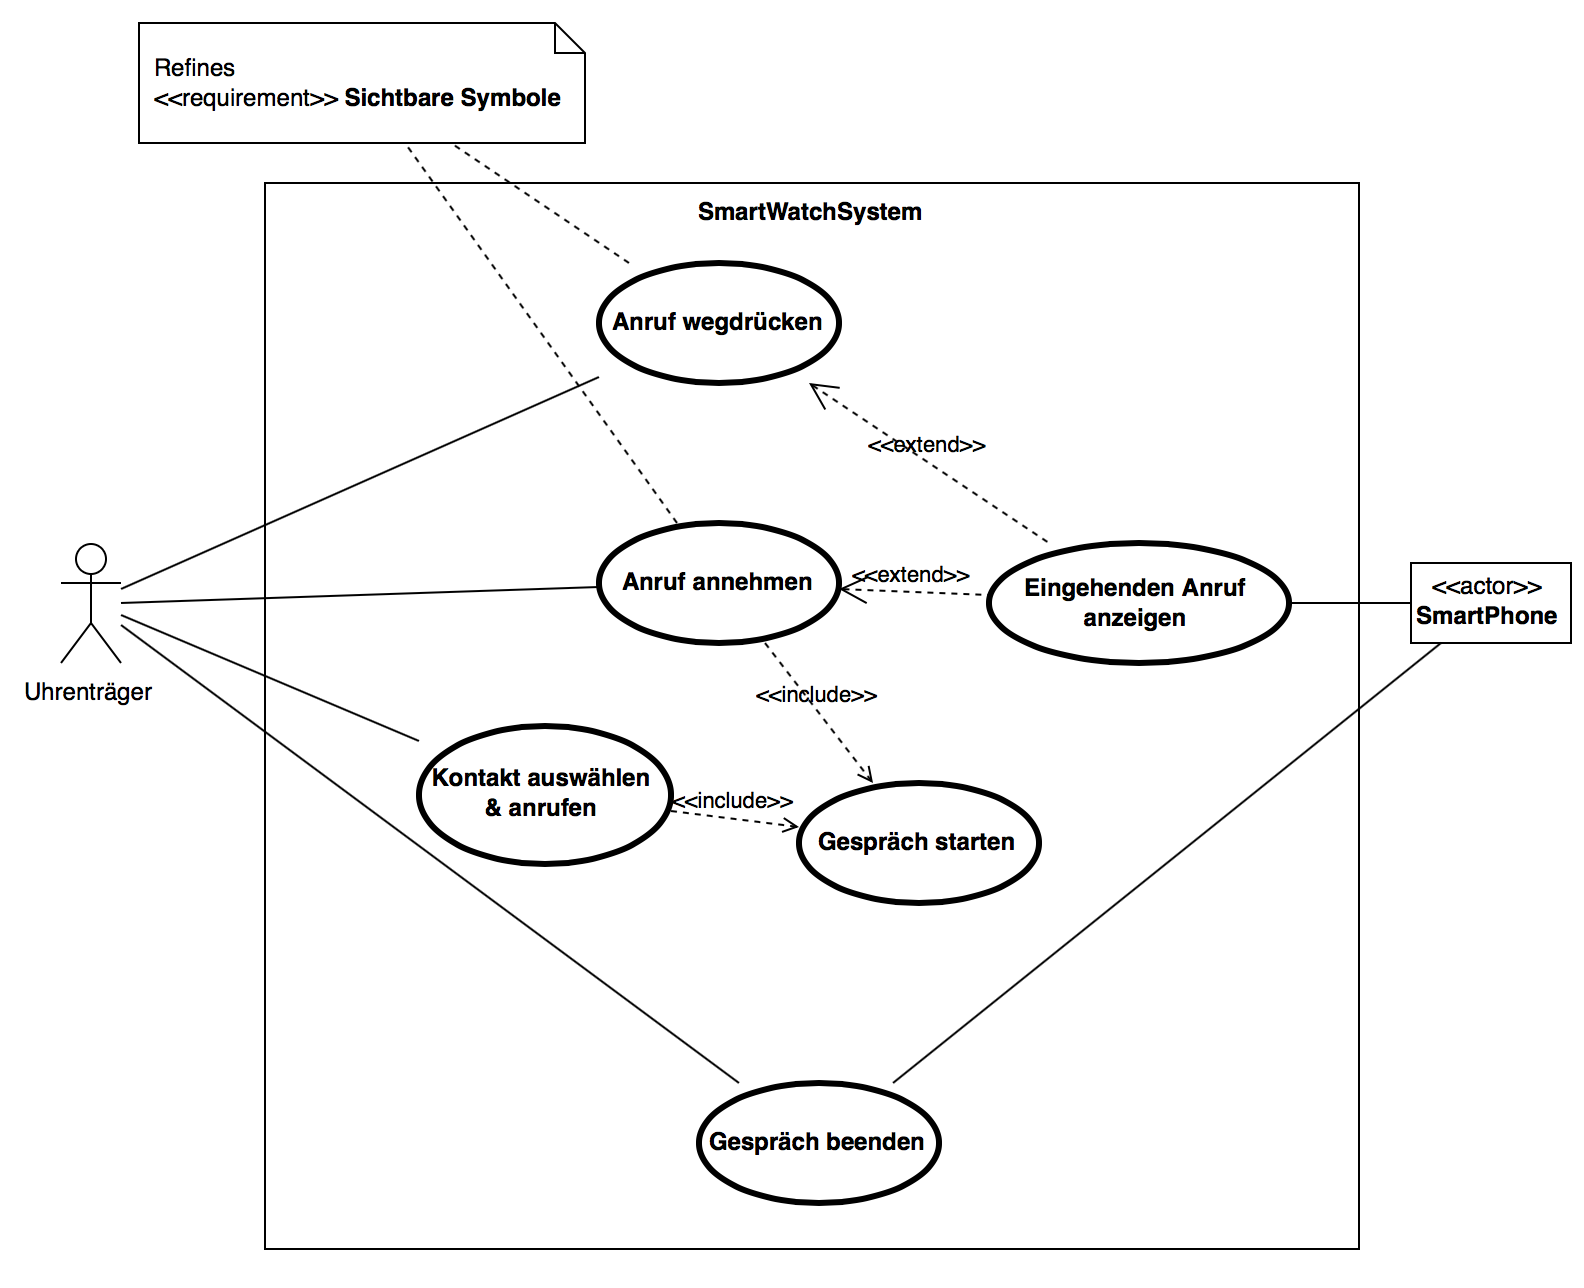
\includegraphics[width=14cm]{img/usecase-anruf-p1}
\caption{Use Case - Anruf}\label{fig:usecase-anruf-p1}
\end{figure}

\begin{figure}[H]
\centering\
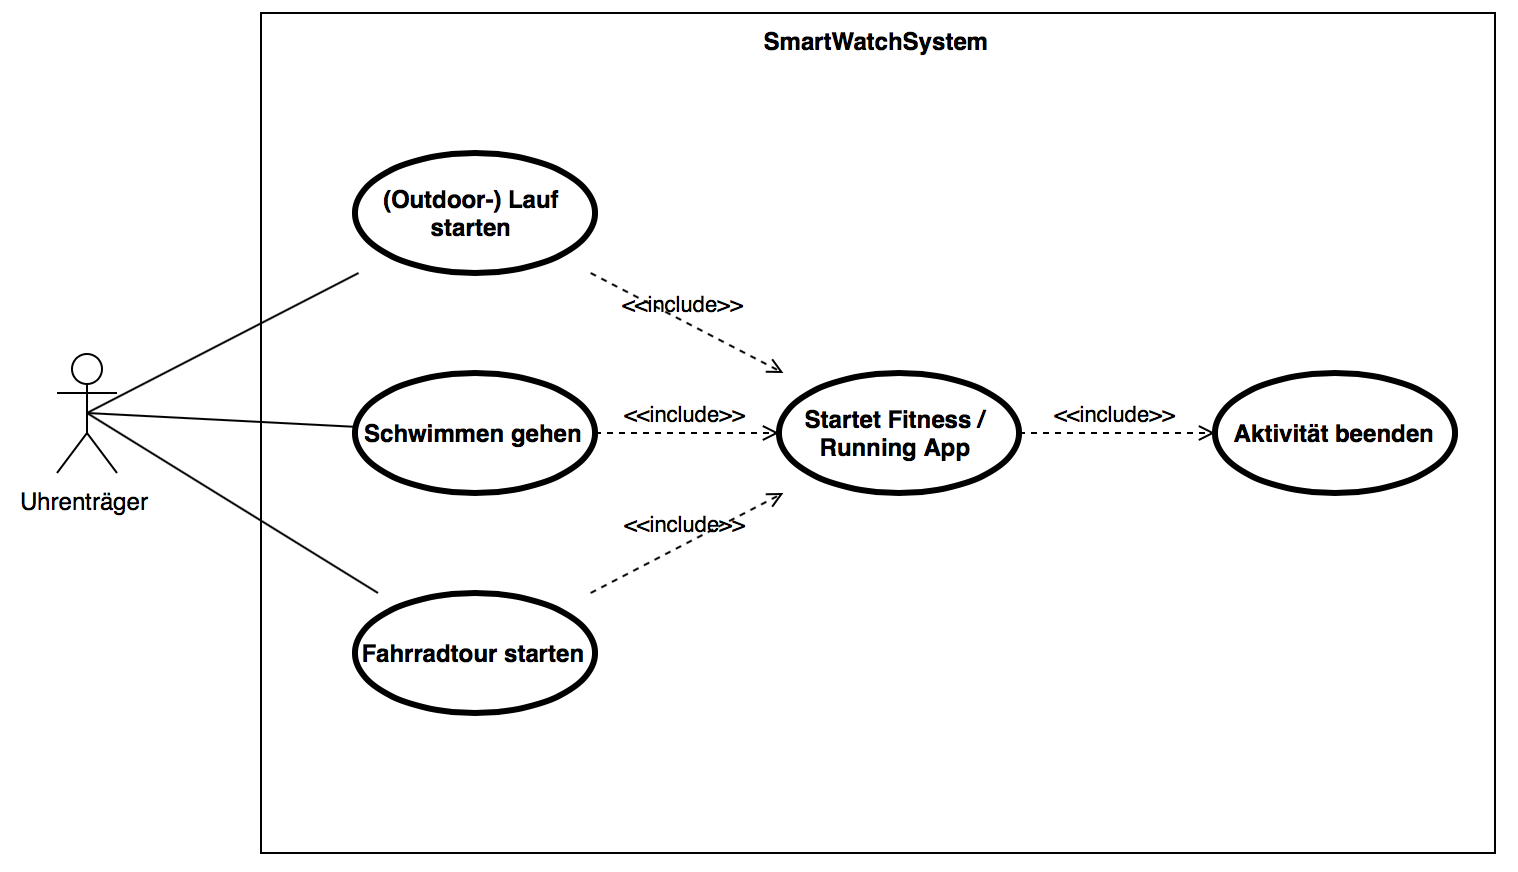
\includegraphics[width=14cm]{img/usecase-fitness-p1}
\caption{Use Case - Fitness}\label{fig:usecase-fitness-p1}
\end{figure}

\begin{figure}[H]
\centering\
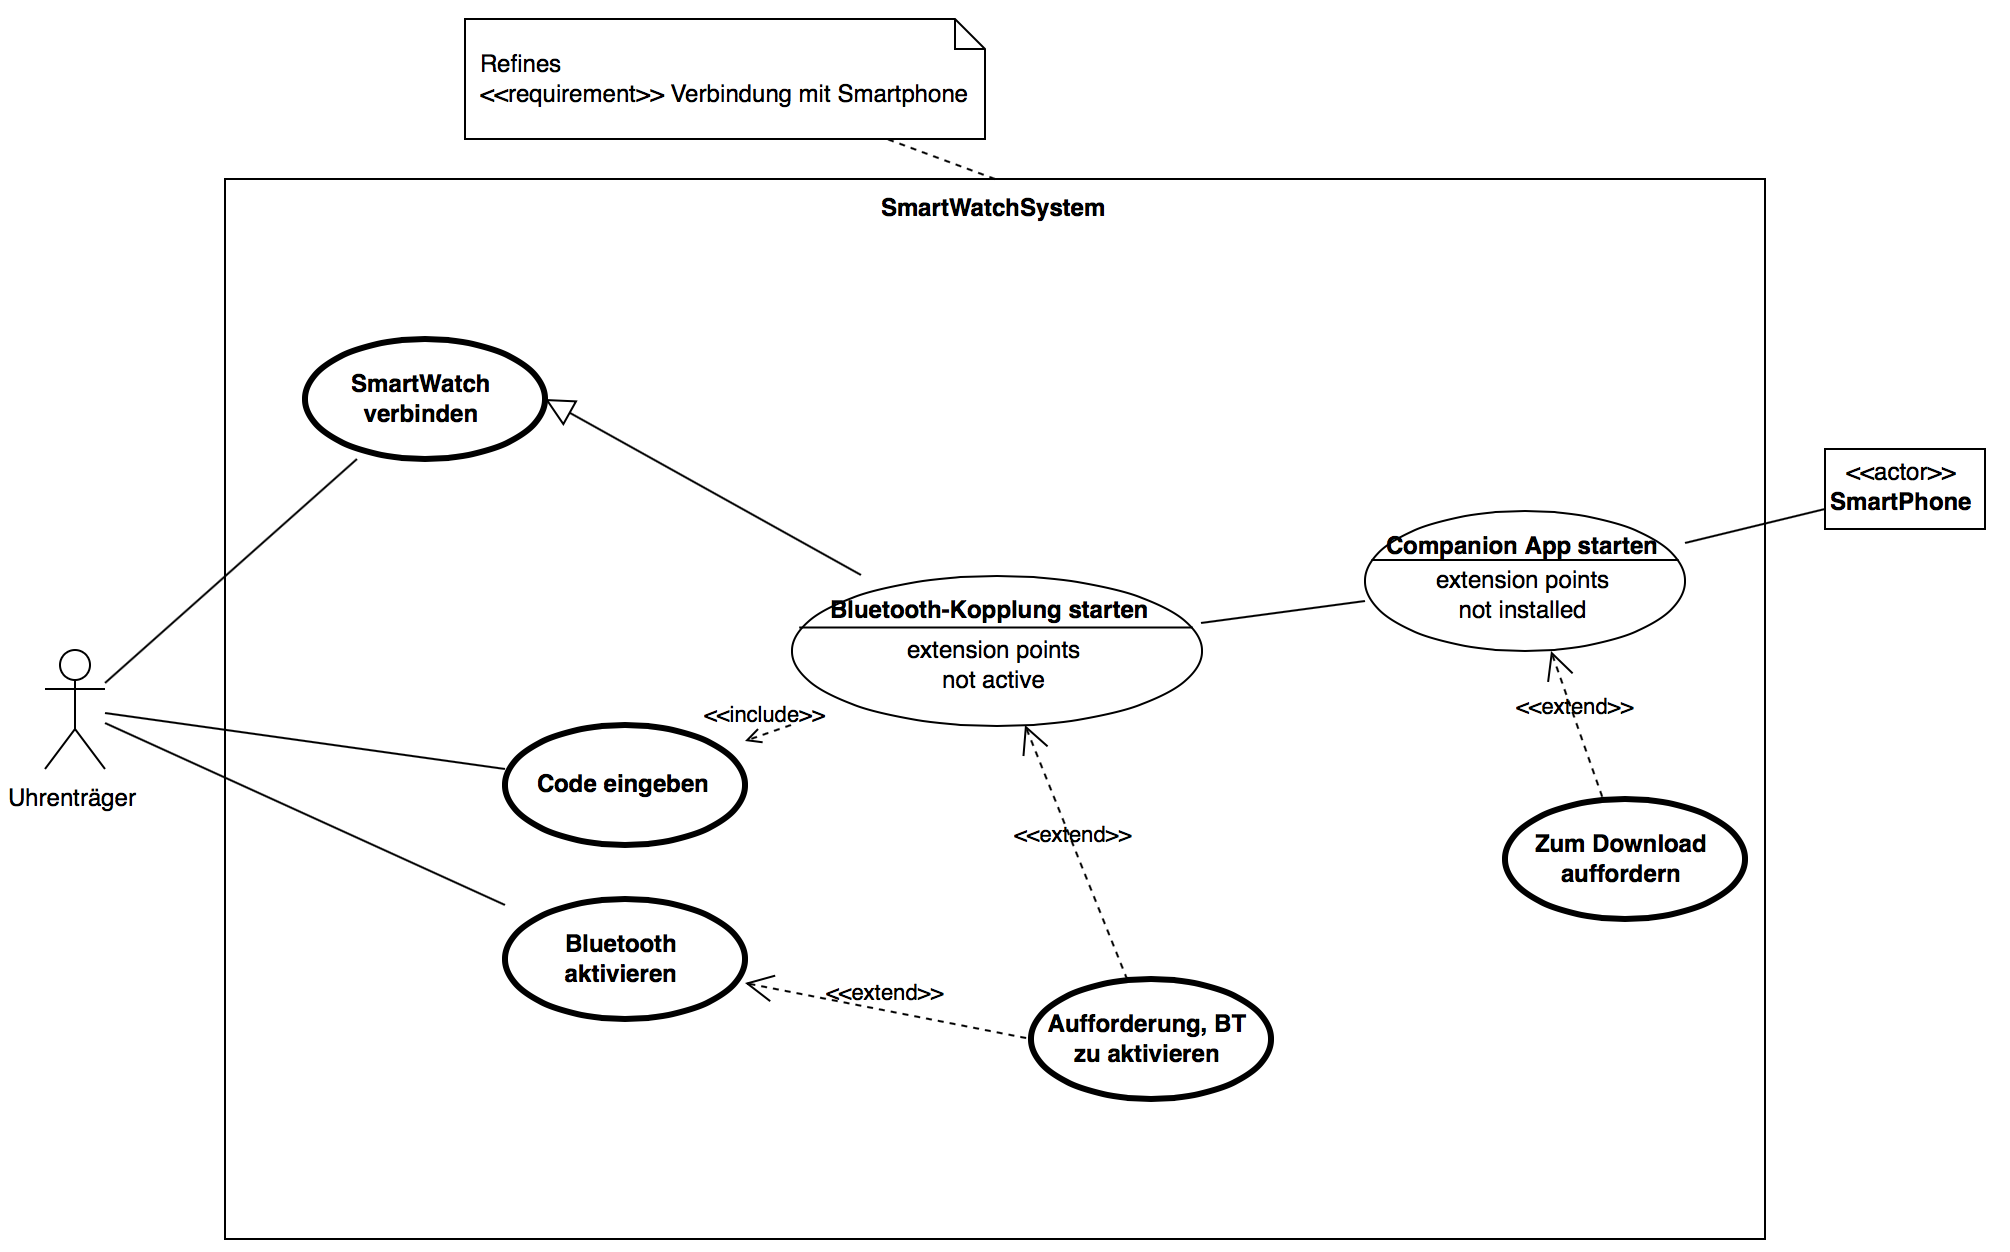
\includegraphics[width=14cm]{img/usecase-pairing-p1}
\caption{Use Case - Pairing}\label{fig:usecase-pairing-p1}
\end{figure}

%% Requirements beschreibung einbinden
\section{Requirements}
Zur Spezifikation\todo{Glossar} der Smartwatch wurden - neben den in Abschnitt~\ref{sec:use_cases} beschriebenen UseCases - die wichtigsten Requirements\todo{Glossar} gesammelt und festgehalten. Um die Übersicht und Nachvollziehbarkeit zu verbesseren, werden diese in die folgenden Kategorien eingeteilt:

\begin{itemize}
	\item Ausgabe -- Ausgabe beinhaltet alle Requirements, die sich auf die grafische und auf die akkustische Ausgabe beziehen.
	\item Usability\todo{Glossar} -- Alle Requirements zur Beschreibung der Bedienbarkeit der Smartwatch
	\item Kapazität -- Alle Requirements bezüglich der Energieversorgung
	\item Funktionen -- Funktionen beinhaltet alle Requirements, die konkrete Funktionen der Smartwatch beschreiben
	\item Ergonomie\todo{Glossar} -- Ergonomische Requirements beschreiben das Design und die physische Eigenschaften der Smartwatch.
\end{itemize}

Das Package-Diagram in Abbildung~\ref{fig:package_diagram_requirements} teilt die Requirements-Kategorien in einzelne Packages\todo{Glossar} auf.

\begin{figure}[H]
\centering\
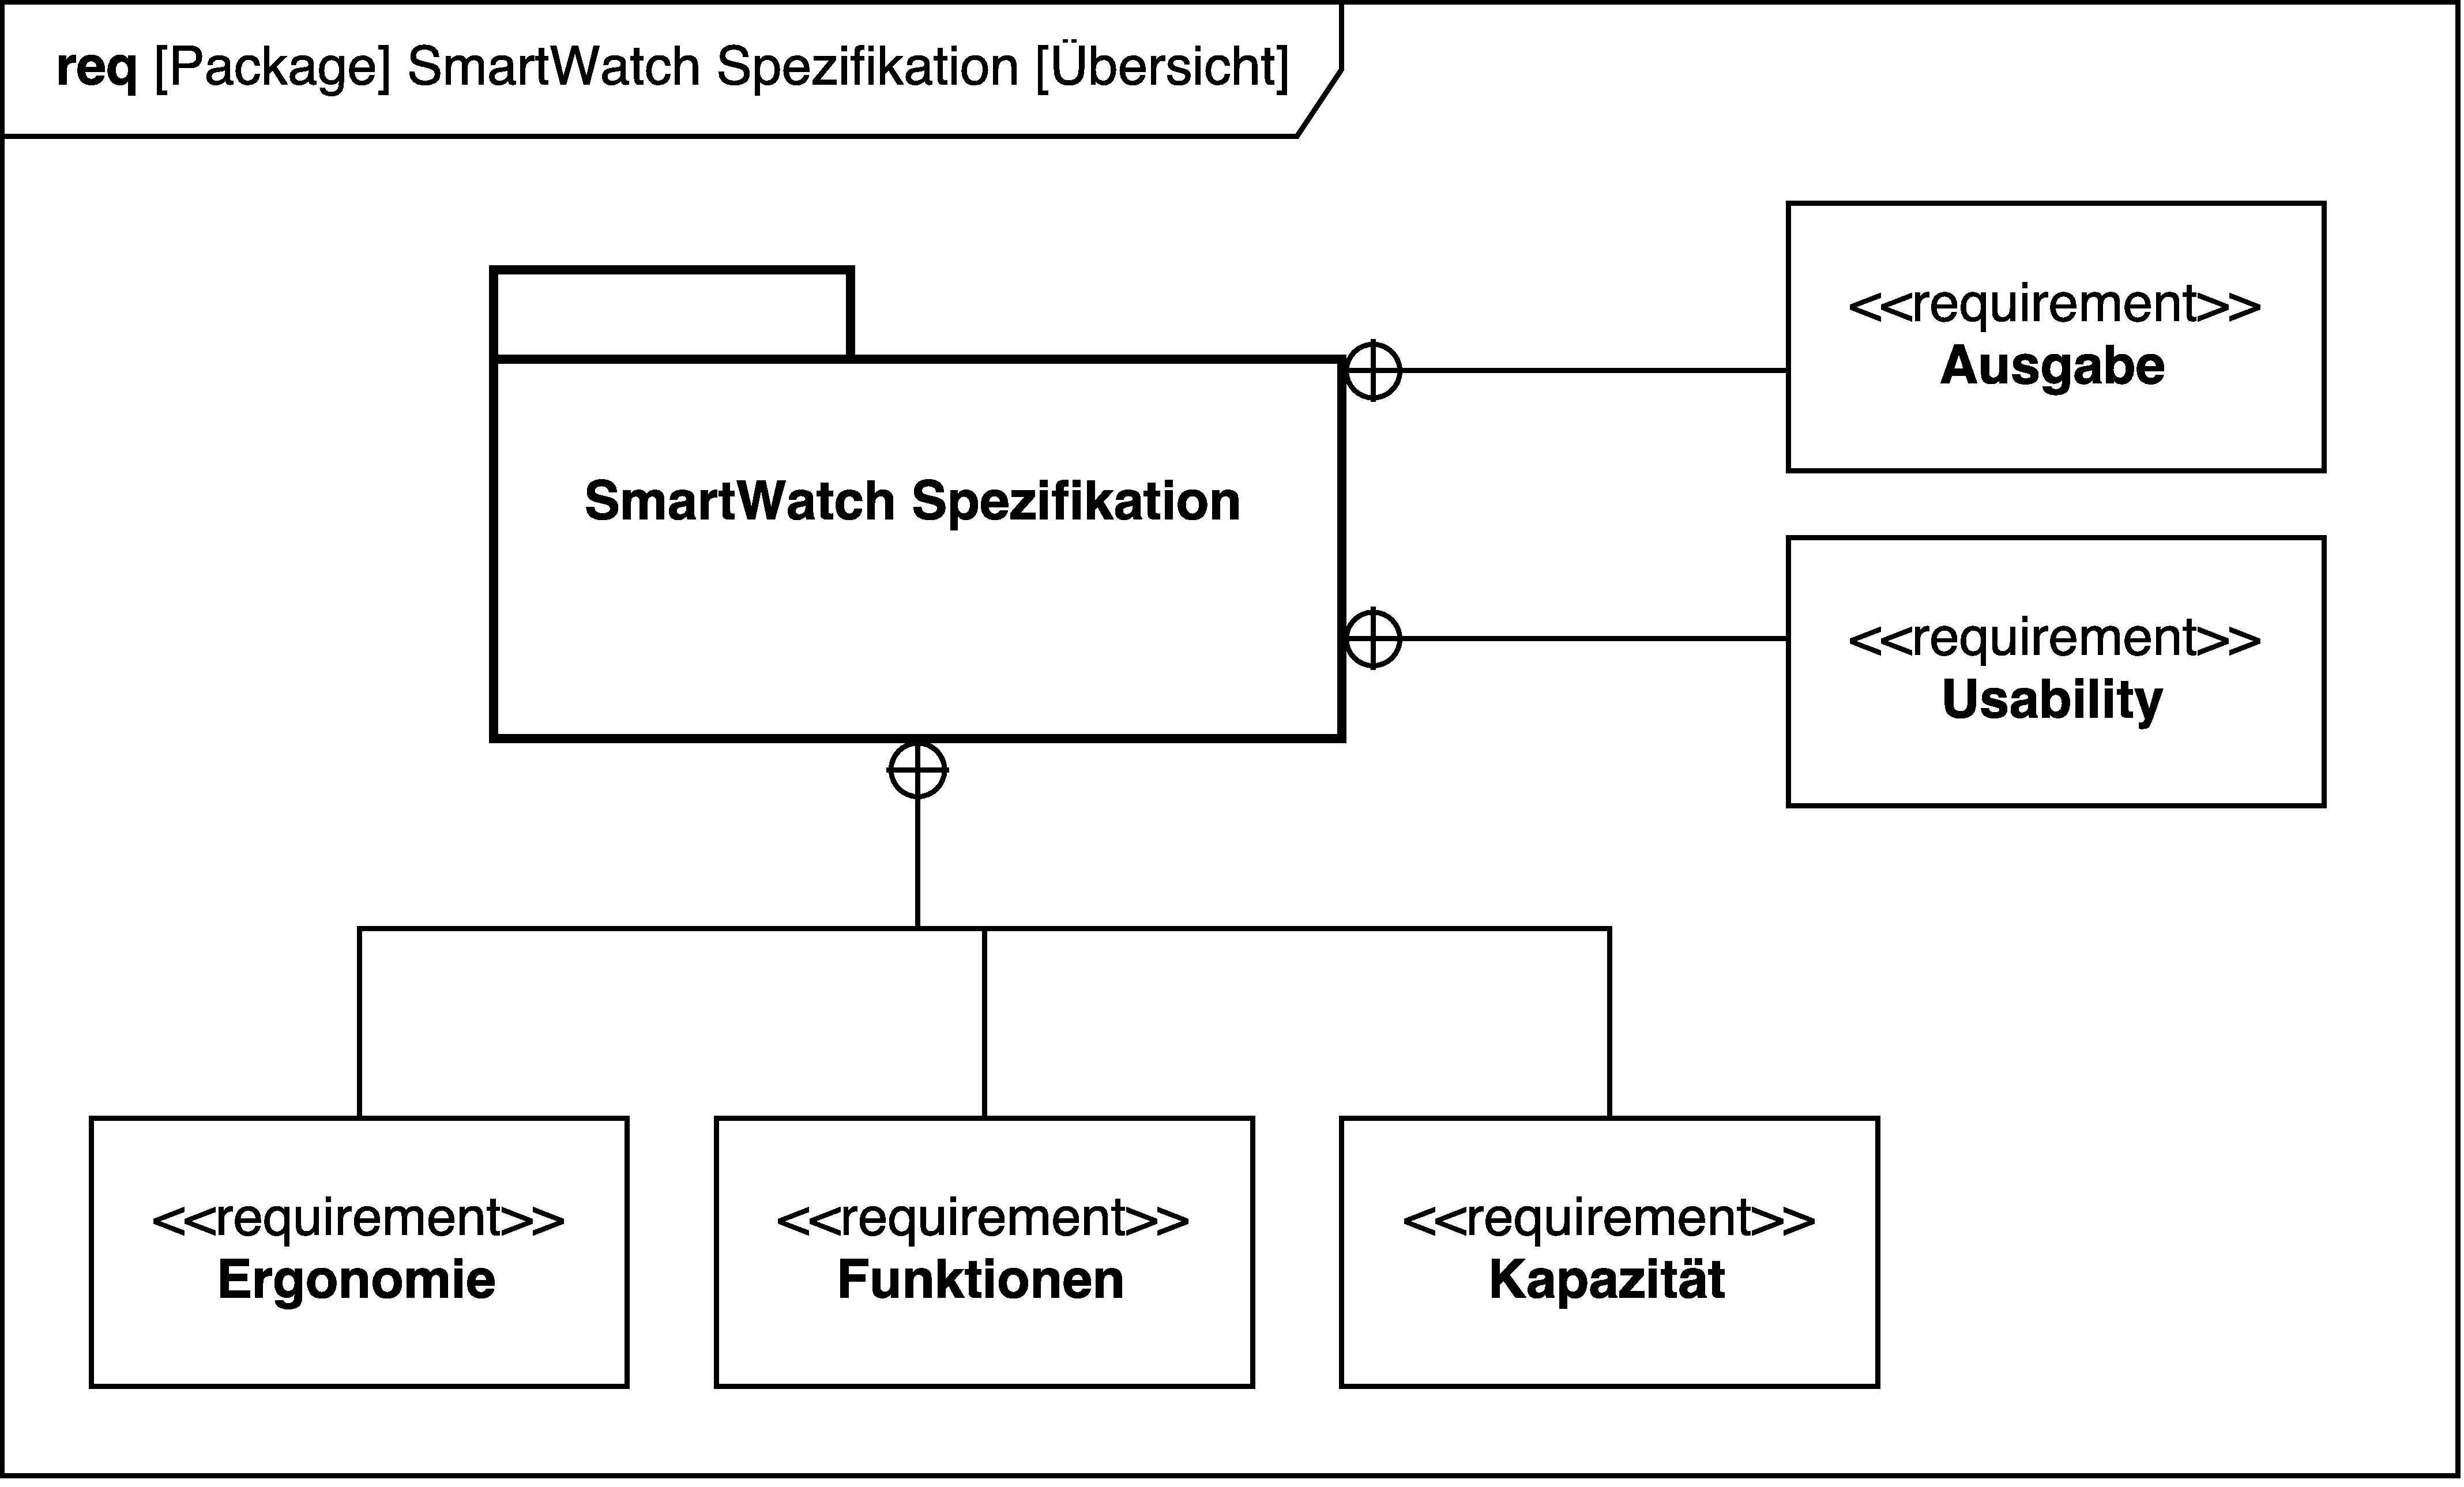
\includegraphics[width=14cm]{img/package_diagram_smartWatch_requirements}
\caption[Requirements: Package Diagram]{Package Diagram der einzelnen Requirement-Kategorien}\label{fig:package_diagram_requirements}
\end{figure}

Tabelle~\ref{tab:table_requirements} enthält die gesammelten Requirements aufgeteilt in die einzelnen Kategorien.

\begin{center}
	\begin{longtable}{|L{2cm}|L{3cm}|L{8.5cm}|}
		\caption[Liste der Requirements]{Auflistung der gesammelten Requirements der Smartwatch} \label{tab:table_requirements} \\
		\hline \multicolumn{1}{|c|}{\textbf{ID}} & \multicolumn{1}{c|}{\textbf{Name}} & \multicolumn{1}{c|}{\textbf{Text}} \\ \hline
		\endfirsthead

		\multicolumn{3}{c}%
		{{\bfseries \tablename\ \thetable{} -- Fortsetzung von vorheriger Seite}} \\
		\hline \multicolumn{1}{|c|}{\textbf{ID}} & \multicolumn{1}{c|}{\textbf{Name}} & \multicolumn{1}{c|}{\textbf{Text}} \\ \hline
		\endhead

		\hline \multicolumn{3}{|r|}{{Fortgesetzt auf der nächsten Seite}} \\ \hline
		\endfoot

		\hline \hline
		\endlastfoot

		%% Ausgabe
		\multicolumn{3}{|l|}{\textbf{Ausgabe}} \\ \hline
		Ausgabe.01 & Displaygröße & Das Display soll eine Auflösung von 500x500 bei einer Bildschirmdiagonale von 4cm besitzen \\ \hline
		Ausgabe.02 & Farbdisplay & Das Display soll Farben darstellen können \\ \hline

		%% Usability
		\multicolumn{3}{|l|}{\textbf{Usability}} \\ \hline
		Usability.01 & Sichtbare Symbole &	Symbole sollten auf dem Display gut erkennbar sein \\ \hline
		Usability.02 & Touch-Symbolgröße &	Symbole, die eine Touch-Funktionalität besitzen, müssen mindestens 75\% des Bildschirms einnehmen \\ \hline

		%% Kapazität
		\multicolumn{3}{|l|}{\textbf{Kapazität}} \\ \hline
		Akku.01 & Akkulaufzeit & Eine Akkuladung soll bei normaler Benutzung mindestens 24 Stunden halten \\ \hline
		Akku.02 & Akkuladezeit & Der Akku soll innerhalb von 2 Stunden vollständig geladen werden \\ \hline
		Akku.03 & Induktionsladen & Der Akku soll über Induktion (z.B. Qi-Standard) geladen werden können \\ \hline

		%% Funktionen
		\multicolumn{3}{|l|}{\textbf{Funktionen}} \\ \hline
		Boot.01 & Bootvorgang maximal 10 Sekunden & Der Bootvorgang der Smartwatch soll maximal 10 Sekunden dauern \\ \hline
		Connection.01 &	Verbindung mit Smartphone & Das System soll sich mit einem Smartphone verbinden können \\ \hline
		Wasserdicht.01 & Wasserdicht bis 30 Meter & Das System soll Wasserdicht bis 30 Meter sein \\ \hline
		Notification.01 & Anzeigen der Notifications & Notifications sollen auf der Uhr angezeigt werden \\ \hline
		Notification.02 & Notifications innerhalb einer Sekunde anzeigen & Notifications sollen maximal nach einer Sekunde auf der Uhr angezeigt werden \\ \hline
		Connection.02 &	Verbindung mit Smartphone in 4 Sekunden & Die Verbindung mit dem Smartphone  muss in maximal 4 Sekunden hergestellt werden \\ \hline

		%% Ergonomie
		\multicolumn{3}{|l|}{\textbf{Ergonomie}} \\ \hline
		Ergonomie.01 & Auswechselbares Armband & Das Armband der Uhr soll ausgewechselt werden können \\ \hline
		Ergonomie.Gewicht.01 & Gesamtgewicht & Das Gesamtgewicht der Uhr soll maximal 50 Gramm wiegen \\ \hline

	\end{longtable}
\end{center}


\section{Package Diagram}
Um die Struktur des Smartwatches zu gliedern und so Schichten in verschieden Abstraktionen
einzuführen werden Paketdiagramme verwendet.
Der Smartwatch wurde dabei in funktionalen und logischen Einheiten zerlegt und in dem jeweiligen Paket zugeordnet.
Über die rein funktionalen Eigenschaften des Systems werden auch die nicht-funktionalen Anforderungen des Smartwatches in Pakete definiert.


Die Abbildung ~\ref{fig:package} beschreibt die Pakete des Smartwatches.
\begin{figure}[H]
\centering\
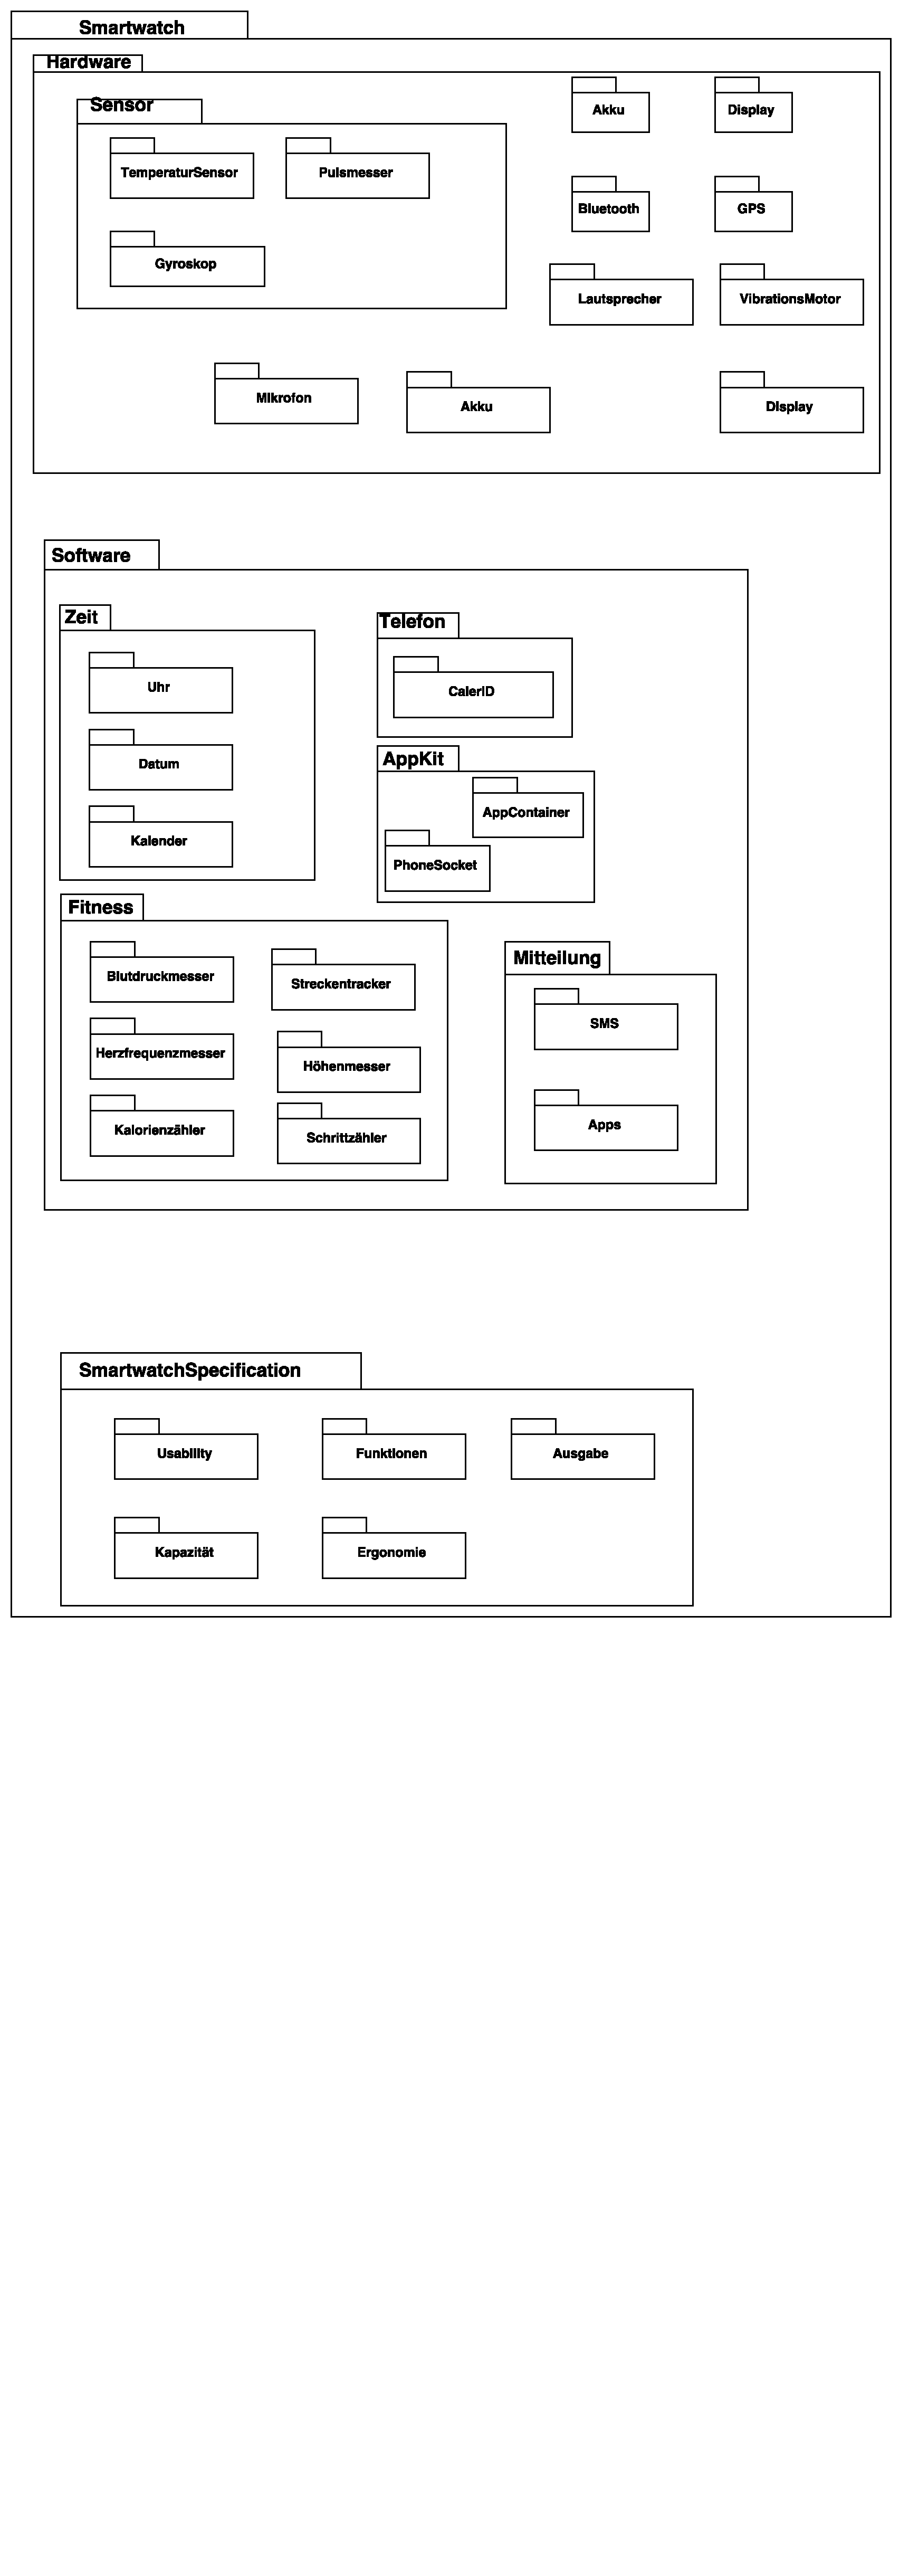
\includegraphics[width=8cm]{img/package}
\caption{Packetdiagramm}\label{fig:package}
\end{figure}

Die Elemente des Pakets Smartwatch sind wiederum Pakete, welche die verschiedenen funktionalen Zuständigkeiten innerhalb des Pakets SmartWatch beschreiben.
Der Smartwatch-Paket ist in Hardware, Software und den nicht-funktionalen Anforderungen
gegliedert (\textit{SmartWatchSpecification}).
Für die Verbindung sorgt Bluetooth 4.0.
Als Sensoren kommen ein Schrittzähler, ein Pulsmesser, Temperatursensor und Gyroskop zum Einsatz. Für die Verbindung sorgt Bluetooth 4.0.
Die Sensoren können z.B zur Aktivitätserkennung.
Der Smartwatch besitz ein Display, auf dem dann wichtige Infos wie Anrufernummer und Benachrichtigungen und die Uhrzeit angezeigt werden.
Die weiteren Hardwarebausteine sind im Package \textit{Hardware} zu finden.

Standard Anwendungen die mit dem Smartwatch geliefert werden, sind Uhrzeitangaben, Erinnerungsfunktionen, Kalender Funktionalität, Benachrichtigungen oder die Aktivitätserkennung. Klassische Anwendungen sind auch die Fitnessfunktionalitäten.
Mit der mitegelieferten API \textit{AppKit} lassen sich Apps für die SmartWatch programmieren, die eng mit dem Smartpohone zusammenarbeiten.
Die softwaretechnische Paketstruktur ist im Package \textit{Software} abgebildet.

\section{Block Definition Diagram}

Das Block Definition Diagram (siehe Abb. \ref{fig:block1}) in dieser Phase stellt den groben, physikalischen Aufbau der \textit{Smartwatch} dar. Diese setzt sich zusammen aus \textit{Sensoren}, einem \textit{Display}, einem \textit{Speichermedium}, einem \textit{Armband}, einen \textit{Gyroskop}, einer \textit{Bluetooth-Antenne} und einem \textit{GPS-Modul}. Um die Stromversorgung der Uhr zu garantieren, soll das \textit{Armband} aus mehreren \textit{Akkuzellen} bestehen. Das \textit{Display} soll dabei komplett von dem \textit{Armband} trennbar sein. So kann die Uhr bei schwachen Akku oder bei einem Wechsel zu einer sportlichen Tätigkeit einfach in einem anderen \textit{Armband} eingesetzt werden. Für die Smartwatch wird das \textit{Gewicht in Gramm}, die \textit{Abmessungen in Millimetern} und die \textit{Auflösung des Displays in Zoll} angegeben. Für das \textit{Armband} wird das \textit{Gewicht in Gramm}, der \textit{Umfang des Bandes in Zentimetern} und die \textit{Farbe} angegeben. Die Akkuleistung wird in Watt beschrieben. Die \textit{Bluetooth-Antenne} soll die Verbindungsstelle zum \textit{Smartphone} sein. Um die Akkulaufzeit zu erhöhen soll die \textit{Antenne}, zusätzlich zum normalen Bluetooth, auch \textit{"Low-Energy" -Bluetooth} unterstützen. Die Smartwatch selbst soll keine Daten, außer die für die Nutzung reiner Sportaktivitäten benötigten, speichern können. Daher ist der \textit{Speicher} recht klein gehalten und dient nicht zum verwalten von Bildern oder anderen Benutzerdaten.
Zu diesem Zeitpunkt der Entwicklung waren die Funktionalitäten noch nicht fertig festgelegt und deshalb fehlen im Diagramm unter anderem die Tasten für das Skalieren und Weiterblättern des Bildschirms und eine genauere Spezifikation der Sensoren.

\begin{figure}[htb]
\centering\
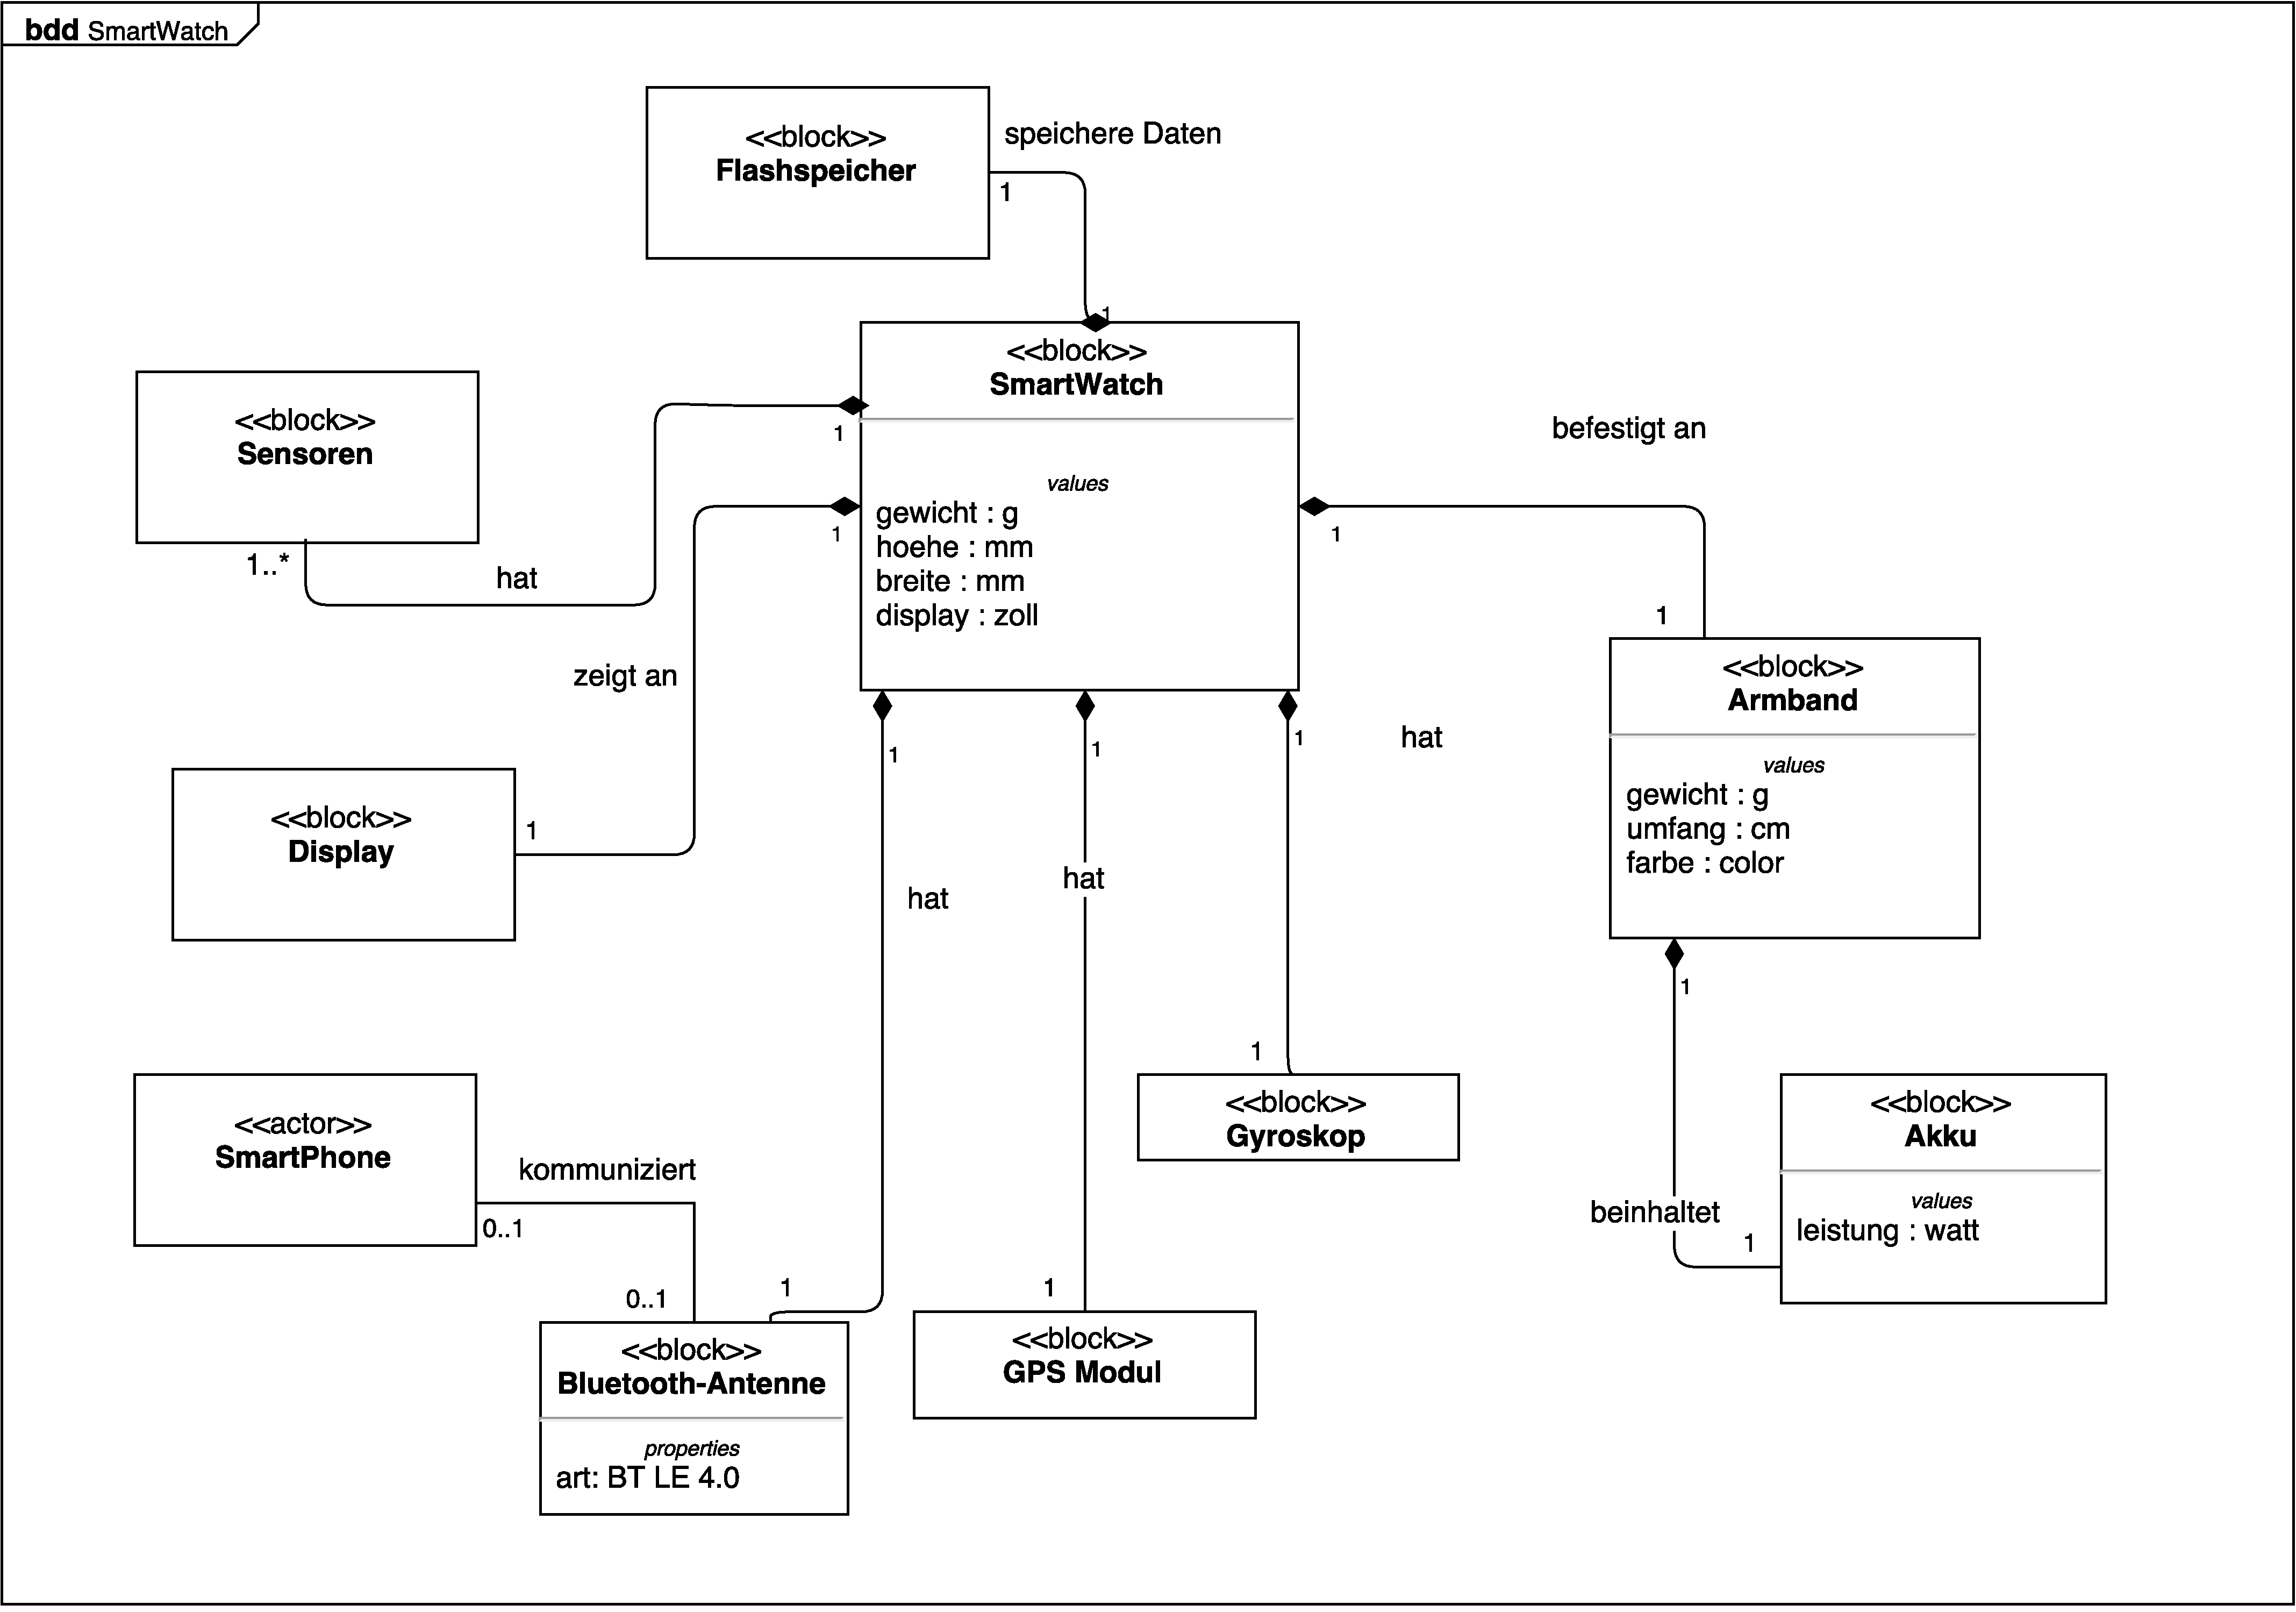
\includegraphics[width=\textwidth]{img/block1}
\caption{Erstes Blockdefinitionsdiagramm für den physikalischen Aufbau der Smartwatch.}\label{fig:block1}
\end{figure}